\section{Лема за покачването}

\begin{lemma}[за покачването (безконтекстни езици)]
  \index{лема за покачването!безконтекстни езици}
  \label{lem:pumping-context} 
  \marginpar{\cite[стр. 125]{sipser3}, \cite[стр. 125]{hopcroft1}, \cite[стр. 148]{kozen}}
  За всеки безконтекстен език $L$ съществува $p>0$, такова
  че ако $\alpha\in L$, за която $\abs{\alpha} \geq p$, то съществува разбиване на думата на пет части, $\alpha=xyuvw$,
  \marginpar{Ще казваме, че $p$ е константа на покачването}
  за което е изпълнено:
  \begin{enumerate}[1)]
  \item
    $\abs{yv}\geq 1$,
  \item
    $\abs{yuv}\leq p$, и
  \item
    $(\forall i\geq 0)[xy^iuv^iw\in L]$.
\end{enumerate}
\end{lemma}
\begin{proof}
  Нека $G$ е граматиката за езика $L$. Да положим
  \[b = \max\{\ |\gamma| \mid A \to \gamma \text{ е правило в }G\ \}.\]
  Нека
  \[p = b^{\abs{V} + 1}.\]
  Ще покажем, че $p$ е константа на покачването за граматиката $G$.
  
  Да разгледаме произволна дума $\alpha \in \L(G)$, за която $\abs{\alpha} \geq p$.
  Понеже $\L(G)$ е безкраен език, то такива думи съществуват.
  Тогава от \Cor{tree:upper-bound} следва, че ако $P = (T,\lambda)$ е дърво на извод за $\alpha$ в $G$, за което $X_\varepsilon = S$, то
  \[b^{|V| + 1}\leq |\alpha| \leq b^{\texttt{height}(T)}.\]
  Оттук следва, че
  \[|V| + 1 \leq \texttt{height}(T).\]
  Нека измежду всички дървета на извод $P = (T,\lambda)$ за $\alpha$ в граматиката $G$ сме избрали такова с минимален брой елементи на $T$.
  Да фиксираме максимален път $\pi$ в $T$, т.е. дума $\pi \in T$ и $|\pi| = \texttt{height}(T)$.
  Ясно е, че
  \marginpar{Броят на върховете по пътя $\pi$ е 1 + броя на ребрата.}
  \[|V| + 1 \leq |\{ X_\gamma \mid \gamma \prec \pi\}| = \texttt{height}(T).\]
  Тук нарочно не броим $X_\pi$, защото $X_\pi \in \Sigma$, а ние се интересуваме само от променливите.
  От принципа на Дирихле следва, че съществува $\beta \prec \pi$, за което
  \begin{equation}
    \label{eq:10}
    X_\beta \in \{X_\gamma \mid \beta \prec \gamma \prec \pi\}.
  \end{equation}
  Нека $\beta$ е най-дългата дума, за която е изпълнено свойството (\ref{eq:10}).
  Да означим с $\gamma$ една от думите, за която $\beta \prec \gamma \prec \pi$ и $X_\gamma = X_\beta$.
  От избора на $\beta$ следва, че
  \begin{equation}
    \label{eq:11}
    \texttt{height}(T_\beta) = |\{ X_\gamma \mid \beta \preceq \gamma \prec \pi\}| \leq |V| + 1,
  \end{equation}
  защото ако допуснем противното, то ще имаме, че $|\{ X_\gamma \mid \beta \prec \gamma \prec \pi\}| \geq |V| + 1$ и от принципа на Дирихле ще следва, че
  съществува по-дълга от $\beta$ дума, за която е изпълнено свойството (\ref{eq:10}).
  
  Нека $u = \texttt{yield}(P_\gamma)$. Тогава $yuv = \texttt{yield}(P_\beta)$, за някои думи $y,v \in \Sigma^\star$.
  Това означава, че думата $\alpha$ може да се запише като $\alpha = xyuvw$, за някои $x, w \in \Sigma^\star$.
  % \marginpar{По пътя $\pi$ е възможно да срещнем много различни двойки повтарящи се променливи, ние избрахме възможно най-долната.}
  Освен това имаме свойствата:
  \begin{enumerate}[1)]
  \item
    Да видим първо защо $\abs{yv}\geq 1$.
    Ако допуснем, че $|yv| = 0$, то това означава, че $\alpha = xuw$ и тази дума
    би имала дърво на извод $(P \setminus P_\beta) \odot P_\gamma$, защото:
    \begin{itemize}
    \item 
      $\texttt{yield}(P_\gamma) = u$;
    \item
      $\texttt{yield}(P \setminus P_\beta) = x X_\beta w$;
    \item
      $X_\alpha = X_\beta$.
    \end{itemize}
    Но това противоречи на избора на $P$ като дървото на извод за думата $\alpha$ с минимален брой елементи в $T$.
  \item
    $\abs{yuv} \leq p$, защото $yuv = \texttt{yield}(T_\beta)$ и оттук следва, че:
    \begin{align*}
      \abs{yuv} & \leq b^{\texttt{height}(T_\beta)} & \comment\text{от \Cor{tree:upper-bound}}\\
                & \leq b^{|V|+1} & \comment\text{от (\ref{eq:11})}\\
                & = p
    \end{align*}
  \item
    Остана само да видим защо за всяко естествено число $i$ е изпълнено, че $xy^iuv^iw \in L$.
    Това е най-сложното разсъждение в лемата, затова нека да го разгледаме внимателно.
    Понеже $\beta \prec \gamma$, нека $\rho$ е тази дума, за която $\gamma = \beta \cdot \rho$.
    Ясно е, че $P_\gamma = (P_\beta)_\rho$ и $P_\beta\setminus (P_\beta)_\rho = (P\setminus P_\gamma)_\beta$.
    \begin{itemize}
    \item
      \marginpar{Да напомним, че $X_\beta \df \lambda(\beta)$.}
      Нека $i = 0$. Тогава $xy^0uv^0w = xuv$ има дърво на извод $(P \setminus P_\beta ) \odot P_\gamma$,
      защото от избора на $\gamma$ и $\beta$ имаме, че:
      \begin{itemize}
      \item 
        $\texttt{yield}(P_\gamma) = u$;
      \item
        $\texttt{yield}(P \setminus P_\beta) = x X_\beta w$;
      \item
        $X_\alpha = X_\beta$.
      \end{itemize}
    \item
      Нека $i = 1$.
      Ясно е от условието, че $xyuvw \in L$, но нека да направим наблюдението, че дървото на извод $P$ за думата $\alpha$ в $G$
      може да се запише и така:
      \[P = (P \setminus P_\beta) \odot (P \setminus P_\gamma)_\beta \odot P_\gamma, \]
      защото:
      \begin{itemize}
      \item
        $\texttt{yield}(P\setminus P_\beta) = x X_\beta w$;
      \item
        $\texttt{yield}((P \setminus P_\gamma)_\beta) = y X_\gamma v$, защото $X_\gamma = \lambda(\gamma) = \lambda_\beta(\rho)$;
      \item
        $\texttt{yield}(P_\gamma) = u$;
      \item
        $X_\beta = X_\gamma$.
      \end{itemize}

      \begin{figure*}[h!]

        \begin{subfigure}[t]{0.5\textwidth}
          \centering

          \begin{tikzpicture}
            \coordinate (A) at (0,0);
            \coordinate (B) at (-2,-2.5);
            \coordinate (C) at (2,-2.5);
            \coordinate (D) at (-1.4,-2.5);
            \coordinate (E) at (-0.7,-2.5);
            \coordinate (F) at (0.7,-2.5);
            \coordinate (G) at (1.4,-2.5);
            
            \coordinate (H) at (0,-0.8);
            \coordinate (I) at (0,-1.5);
            
            
            \draw (A) -- node[left]{$\scriptstyle{T\ =\ }$}(B) -- (C) -- (A);
            \draw (H) -- (D) -- (G) -- (H);
            \draw (I) -- (E) -- (F) -- (I);
            
            \draw [photon] (A) -- node[below left]{$\scriptstyle{\beta}$} (H);
            \draw [photon] (H) -- node[below left]{$\scriptstyle{\rho}$} (I);
          \end{tikzpicture}
        \end{subfigure}
        % \hskip 0.1in
        $\stackrel{\lambda}{\Rightarrow}$
        % \hskip 0.1in                  
        \begin{subfigure}[t]{0.5\textwidth}
          \centering
          
          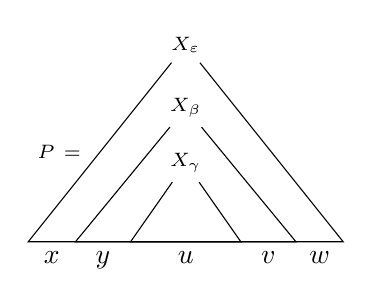
\begin{tikzpicture}
            \node (A) at (0,0) {${\scriptstyle X_\varepsilon}$};
            \coordinate (B) at (-2,-2.5);
            \coordinate (C) at (2,-2.5);
            \coordinate (D) at (-1.4,-2.5);
            \coordinate (E) at (-0.7,-2.5);
            \coordinate (F) at (0.7,-2.5);
            \coordinate (G) at (1.4,-2.5);
            
            \node (H) at (0,-0.8) {${\scriptstyle X_\beta}$};
            \node (I) at (0,-1.5) {${\scriptstyle X_\gamma}$};
            
            \draw (A) -- node[left]{$\scriptstyle{P\ =\ }$}(B) -- node[below]{$x$} (D) -- node[below]{$y$}(E) -- node[below]{$u$}(F) -- node[below]{$v$}(G) -- node[below]{$w$}(C) -- (A);
            \draw (H) -- (D) -- (G) -- (H);
            \draw (I) -- (E) -- (F) -- (I);
          \end{tikzpicture}
        \end{subfigure}
      \end{figure*}

      Можем да разбием синтактичното дърво $P$ по следния начин:

      \begin{figure*}[h!]
        \begin{subfigure}[t]{0.5\textwidth}
          \centering
          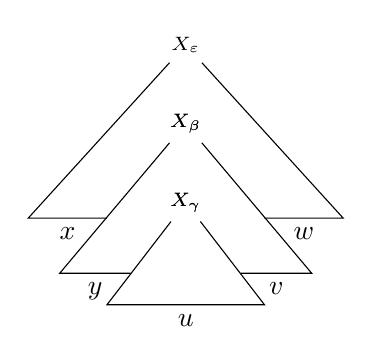
\begin{tikzpicture}
            \node (A) at (0,0) {${\scriptstyle X_\varepsilon}$};
            \coordinate (B) at (-2,-2.2);
            \coordinate (C) at (2,-2.2);
            \coordinate (S) at (-1,-2.2);
            \coordinate (T) at (1,-2.2);
            \node (L) at (0,-1) {${\scriptstyle X_\beta}$};
            
            \coordinate (E) at (-0.7,-2.5);
            \coordinate (F) at (0.7,-2.5);
            
            
            \node (H) at (0,-1) {${\scriptstyle X_\beta}$};
            \node (X) at (0,-2) {${\scriptstyle X_\gamma}$};
            \coordinate (D) at (-1.6,-2.9);
            \coordinate (G) at (1.6,-2.9);
            \coordinate (E) at (-0.7,-2.9);
            \coordinate (F) at (0.7,-2.9);
            
            \node (I) at (0,-2) {${\scriptstyle X_\gamma}$};
            \coordinate (U) at (-1,-3.3);
            \coordinate (V) at (1,-3.3);
            
            \draw (A) -- (B) -- node[below]{$x$}(S);
            \draw (T) -- node[below]{$w$}(C) -- (A);
            \draw (H) -- (D) -- node[below]{$y$}(E);
            \draw (F) -- node[below]{$v$}(G) -- (H);
            \draw (I) -- (U) -- node[below]{$u$}(V) -- (I);
          \end{tikzpicture}
          \caption{$\texttt{yield}((P\setminus P_\beta) \odot (P\setminus P_\gamma)_\beta \odot P_\gamma) = xyuvw$}
        \end{subfigure}
        ~
        \begin{subfigure}[t]{0.5\textwidth}
          \centering
          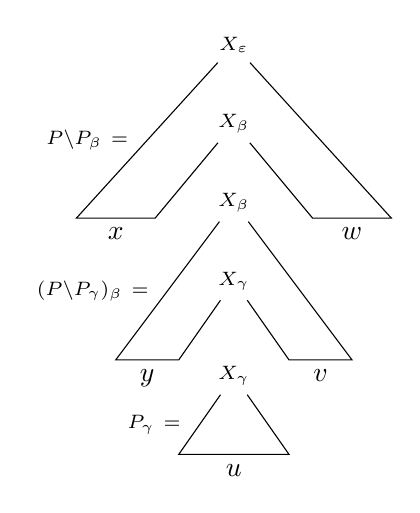
\begin{tikzpicture}
            \node (A) at (0,0) {${\scriptstyle X_\varepsilon}$};
            \coordinate (B) at (-2,-2.2);
            \coordinate (C) at (2,-2.2);
            \coordinate (S) at (-1,-2.2);
            \coordinate (T) at (1,-2.2);
            \node (L) at (0,-1) {${\scriptstyle X_\beta}$};
            
            \coordinate (E) at (-0.7,-2.5);
            \coordinate (F) at (0.7,-2.5);
            
            
            \node (H) at (0,-2) {${\scriptstyle X_\beta}$};
            \node (X) at (0,-3) {${\scriptstyle X_\gamma}$};
            \coordinate (D) at (-1.5,-4);
            \coordinate (G) at (1.5,-4);
            \coordinate (E) at (-0.7,-4);
            \coordinate (F) at (0.7,-4);
            
            \node (I) at (0,-4.2) {${\scriptstyle X_\gamma}$};
            \coordinate (U) at (-0.7,-5.2);
            \coordinate (V) at (0.7,-5.2);
            
            \draw (A) -- node[left]{${\scriptstyle P \setminus P_\beta\ =\ } $}(B) -- node[below]{$x$}(S) -- (L) -- (T) -- node[below]{$w$}(C) -- (A);
            \draw (H) -- node[left]{${\scriptstyle (P\setminus P_\gamma)_\beta\ =\ }$}(D) -- node[below]{$y$}(E) -- (X) -- (F) -- node[below]{$v$}(G) -- (H);
            \draw (I) -- node[left]{${\scriptstyle P_\gamma\ =\ }$}(U) -- node[below]{$u$}(V) -- (I);
          \end{tikzpicture}
          \caption{Можем да разделим $P$ на три части}
        \end{subfigure}
      \end{figure*}
      
      \begin{figure*}[h!]
        \begin{subfigure}[t]{0.5\textwidth}
          \centering
          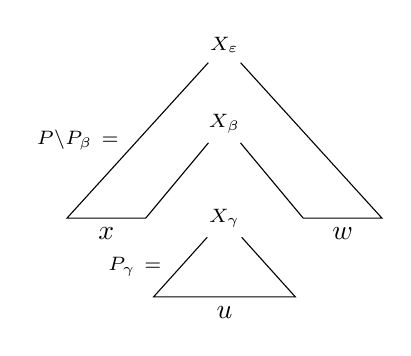
\begin{tikzpicture}
            \node (A) at (0,0) {${\scriptstyle X_\varepsilon}$};
            \coordinate (B) at (-2,-2.2);
            \coordinate (C) at (2,-2.2);
            \coordinate (S) at (-1,-2.2);
            \coordinate (T) at (1,-2.2);
            \node (L) at (0,-1) {${\scriptstyle X_\beta}$};
            
            \coordinate (E) at (-0.7,-2.5);
            \coordinate (F) at (0.7,-2.5);
            
            \coordinate (D) at (-1.5,-4);
            \coordinate (G) at (1.5,-4);
            \coordinate (E) at (-0.7,-4);
            \coordinate (F) at (0.7,-4);
            
            \node (I) at (0,-2.2) {${\scriptstyle X_\gamma}$};
            \coordinate (U) at (-0.9,-3.2);
            \coordinate (V) at (0.9,-3.2);
            
            \draw (A) -- node[left]{${\scriptstyle P \setminus P_\beta\ =\ } $}(B) -- node[below]{$x$}(S) -- (L) -- (T) -- node[below]{$w$}(C) -- (A);
            \draw (I) -- node[left]{${\scriptstyle P_\gamma\ =\ }$}(U) -- node[below]{$u$}(V) -- (I);
          \end{tikzpicture}
          \caption{Понеже $X_\beta = X_\gamma$, можем да махнем средната част пак да получим дърво на извод.}
        \end{subfigure}
        $\stackrel{\scriptstyle{X_\beta = X_\gamma}}{\implies}$
        \begin{subfigure}[t]{0.5\textwidth}
          \centering
          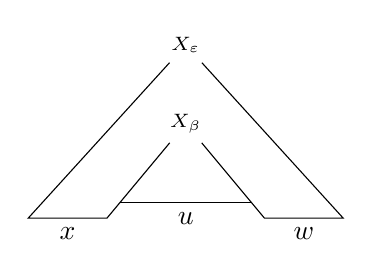
\begin{tikzpicture}
            \node (A) at (0,0) {${\scriptstyle X_\varepsilon}$};
            \coordinate (B) at (-2,-2.2);
            \coordinate (C) at (2,-2.2);
            \coordinate (S) at (-1,-2.2);
            \coordinate (T) at (1,-2.2);
            \node (L) at (0,-1) {${\scriptstyle X_\beta}$};

            \coordinate (U) at (-0.84,-2);
            \coordinate (V) at (0.84,-2);
        
            \draw (A) -- (B) -- node[below]{$x$}(S) -- (L) -- (T) -- node[below]{$w$}(C) -- (A);
            \draw (U) -- node[below]{$u$}(V);
          \end{tikzpicture}
          \caption{$\texttt{yield}((P\setminus P_\beta) \odot P_\gamma) = xuw$}
        \end{subfigure}
      \end{figure*}
      
      Сега вече имаме идея как да обобщим горната конструкция за $i > 1$.
    \item

      \begin{figure*}[h!]
        \begin{subfigure}[t]{0.5\textwidth}
          \centering
          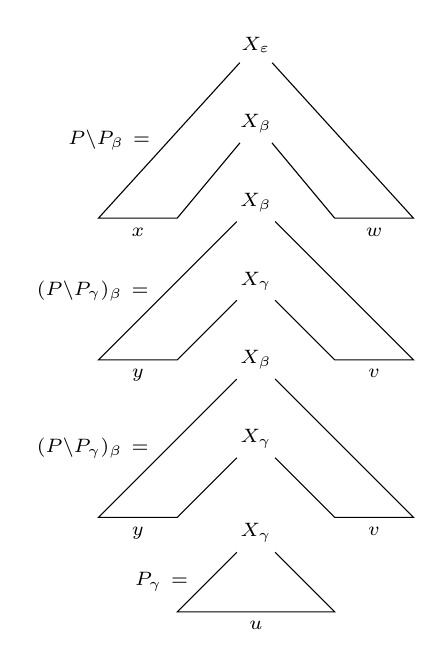
\begin{tikzpicture}
            \node (A) at (0,0) {${\scriptstyle X_\varepsilon}$};
            \coordinate (B) at (-2,-2.2);
            \coordinate (C) at (2,-2.2);
            \coordinate (S) at (-1,-2.2);
            \coordinate (T) at (1,-2.2);
            \node (L) at (0,-1) {${\scriptstyle X_\beta}$};
            
            \coordinate (E) at (-0.7,-2.5);
            \coordinate (F) at (0.7,-2.5);
                        
            \node (H) at (0,-2) {${\scriptstyle X_\beta}$};
            \node (X) at (0,-3) {${\scriptstyle X_\gamma}$};
            \coordinate (D) at (-2,-4);
            \coordinate (G) at (2,-4);
            \coordinate (E) at (-1,-4);
            \coordinate (F) at (1,-4);
            
            \node (H1) at (0,-4) {${\scriptstyle X_\beta}$};
            \node (X1) at (0,-5) {${\scriptstyle X_\gamma}$};
            \coordinate (D1) at (-2,-6);
            \coordinate (G1) at (2,-6);
            \coordinate (E1) at (-1,-6);
            \coordinate (F1) at (1,-6);
            
            \node (I) at (0,-6.2) {${\scriptstyle X_\gamma}$};
            \coordinate (U) at (-1,-7.2);
            \coordinate (V) at (1,-7.2);
            
            \draw (A) -- node[left]{${\scriptstyle P \setminus P_\beta\ =\ } $}(B) -- node[below]{$\scriptstyle{x}$}(S) -- (L) -- (T) -- node[below]{$\scriptstyle{w}$}(C) -- (A);
            \draw (H) -- node[left]{${\scriptstyle (P\setminus P_\gamma)_\beta\ =\ }$}(D) -- node[below]{$\scriptstyle{y}$}(E) -- (X) -- (F) -- node[below]{$\scriptstyle{v}$}(G) -- (H);
            \draw (H1) -- node[left]{${\scriptstyle (P\setminus P_\gamma)_\beta\ =\ }$}(D1) -- node[below]{$\scriptstyle{y}$}(E1) -- (X1) -- (F1) -- node[below]{$\scriptstyle{v}$}(G1) -- (H1);
            \draw (I) -- node[left]{${\scriptstyle P_\gamma\ =\ }$}(U) -- node[below]{$\scriptstyle{u}$}(V) -- (I);
          \end{tikzpicture}
          \caption{Понеже $X_\beta = X_\gamma$, можем да добавим средната част втори път и пак да получим дърво на извод.}
        \end{subfigure}
        $\stackrel{\scriptstyle{X_\beta = X_\gamma}}{\implies}$
        \begin{subfigure}[t]{0.5\textwidth}
          \centering
          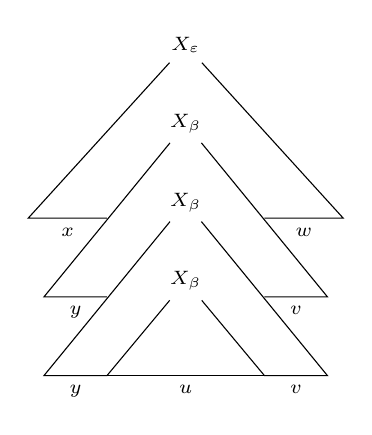
\begin{tikzpicture}
            \node (A) at (0,0) {${\scriptstyle X_\varepsilon}$};
            \coordinate (B) at (-2,-2.2);
            \coordinate (C) at (2,-2.2);
            \coordinate (S) at (-1,-2.2);
            \coordinate (T) at (1,-2.2);
            \node (L) at (0,-1) {${\scriptstyle X_\beta}$};
            
            \coordinate (E) at (-0.7,-2.5);
            \coordinate (F) at (0.7,-2.5);
            
            \node (X) at (0,-2) {${\scriptstyle X_\beta}$};
            \coordinate (D) at (-1.8,-3.2);
            \coordinate (G) at (1.8,-3.2);
            \coordinate (E) at (-1,-3.2);
            \coordinate (F) at (1,-3.2);
            
            \node (X1) at (0,-3) {${\scriptstyle X_\beta}$};
            \coordinate (D1) at (-1.8,-4.2);
            \coordinate (G1) at (1.8,-4.2);
            \coordinate (E1) at (-1,-4.2);
            \coordinate (F1) at (1,-4.2);
            
            \coordinate (U) at (-1,-4.2);
            \coordinate (V) at (1,-4.2);
            
            \draw (A) --  (B)  -- node[below]{$\scriptstyle{x}$}(S);
            \draw (T)  -- node[below]{$\scriptstyle{w}$}(C)  -- (A);
            \draw (L) --  (D)  -- node[below]{$\scriptstyle{y}$}(E);
            \draw (F)  -- node[below]{$\scriptstyle{v}$}(G)  -- (L);
            \draw (X) --  (D1) -- node[below]{$\scriptstyle{y}$}(E1) -- (X1) -- (F1) -- node[below]{$\scriptstyle{v}$}(G1) -- (X);
            \draw (U)  -- node[below]{$\scriptstyle{u}$}(V);
          \end{tikzpicture}
          \caption{$\texttt{yield}((P\setminus P_\beta) \odot (P\setminus P_\gamma)^{(2)}_\beta\odot P_\gamma)$}
        \end{subfigure}
      \end{figure*}
      Нека $i > 1$. Тогава $xy^iuv^iw$ има дърво на извод
      \[(P \setminus P_\beta) \odot ( (P \setminus P_\gamma)_\beta)^{(i)} \odot P_\gamma,\]
      защото:
      \begin{itemize}
      \item
        $\texttt{yield}(P\setminus P_\beta) = x X_\beta w$;
      \item
        $\texttt{yield}((P \setminus P_\gamma)_\beta)^{(i)}) = y^i X_\gamma v^i$ от \Prob{tree:iteration},
        защото $X_\gamma = \lambda(\gamma) = \lambda_\beta(\rho)$;
      \item
        $\texttt{yield}(P_\gamma) = u$;
      \item
        $X_\beta = X_\gamma$.
      \end{itemize}
    \end{itemize}

  \end{enumerate}
\end{proof}

\begin{cor}
  \label{cor:pumping-context-free}
  \marginpar{Ако $L$ е краен език, то е ясно, че $L$ е безконтекстен.}
  Нека $L$ е произволен {\bf безкраен} език. Нека също така е изпълнено, че:
  \begin{description}
  \item[($\forall$)]
    за {\em всяко} естествено число $p \geq 1$,
  \item[($\exists$)]
    можем да намерим дума $\alpha \in L$, $\abs{\alpha}\geq p$, такава че
  \item[($\forall$)]
    за {\em всяко} разбиване на думата на пет части, $\alpha = xyuvw$, със свойствата $\abs{yv} \geq 1$ и $\abs{yuv} \leq p$,
  \item[($\exists$)]
    можем да посочим $i \in \Nat$, за което е изпълнено, че $xy^iuv^iw \not\in L$.
  \end{description}  
  \marginpar{\writedown Докажете! Аналогично е на \Cor{pumping-reg}}
  Тогава $L$ {\bf не} е безконтекстен език.
\end{cor}

\begin{cor}
  \marginpar{\writedown Докажете!}
  Нека $G$ е безконтекстна граматика и $p$ е константата на покачването за $G$.
  Тогава $\abs{\L(G)} = \infty$ точно тогава, когато съществува $\alpha \in \L(G)$, за която $p \leq \abs{\alpha} < 2p$.
\end{cor}
% \begin{proof}
%   Ако съществува дума $\alpha \in L$, за която $\abs{\alpha} \geq p$, то от \Lem{pumping-context} следва,
%   че $\abs{L} = \infty$, защото $\alpha = xyuvw$ и $xy^iuv^iw \in L$, за всяко $i\in\Nat$.

%   За другата посока, нека сега $\abs{L} = \infty$.
%   Да изберем най-късата дума $\alpha \in L$, за която $\abs{\alpha} \geq p$.
%   Ще докажем, че $p \leq \abs{\alpha} < 2p$. За целта да допуснем, че $\abs{\alpha} \geq 2p$.
%   Тогава от \Lem{pumping-context} следва, че $\alpha = xyuvw$, $\abs{yv} \geq 1$, $\abs{yuv} \leq p$, $xy^0uv^0w = xuw \in L$.
%   Ако $\abs{xuw} < p$, то $\abs{yv} > p$, защото $\abs{yv} + \abs{xuw} = \abs{\alpha} \geq 2p$, и следователно $\abs{yuv} > p$, което е противоречие.
%   Следва, че $\abs{\alpha} > \abs{xuw} \geq p$.
%   Получихме, че думата $xuw\in L$ и $\abs{xuw} \geq p$. Това е противоречие с минималността на $\alpha$.
% \end{proof}

% \begin{framed}
%   \Lem{pumping-context} е полезна, когато искаме да докажем, че даден език $L$ {\bf не} е безконтекстен.
%   За целта, доказваме отрицанието на свойствата от \Lem{pumping-context} за $L$, т.е.
%   за всяка константа $p$, ние намираме дума $\alpha \in L$, $\abs{\alpha}\geq p$, такава че за всяко разбиване на думата на пет части, $\alpha = xyuvw$,
%   със свойствата $\abs{yv} \geq 1$ и $\abs{yuv} \leq p$, е изпълнено, че $(\exists i)[xy^iuv^iw \not\in L]$.
% \end{framed}

\begin{remark}
  Алгоритъм за проверка дали един безконтекстен език е безкраен следвайки горния критерий би 
  имал експоненциална сложност относно $|G|$.
\end{remark}

\begin{problem}
  \label{prob:anbncn}
  Докажете, че езикът 
  \[L = \{a^nb^nc^n\ \mid\ n\in\Nat\}\]
  не е безконтекстен.
\end{problem}
\begin{proof}
  \begin{description}
  \item[$(\forall)$]
    Разглеждаме произволна константа $p \geq 1$.
  \item[$(\exists)$]
    Избираме дума $\alpha \in L$, $\abs{\alpha} \geq p$.
    В случая, нека $\alpha = a^pb^pc^p$.
  \item[$(\forall)$]
    Разглеждаме произволно разбиване $xyuvw = \alpha$, за което $\abs{yuv} \leq p$ и $1 \leq \abs{yv}$.
  \item[$(\exists)$]
    Ще изберем $i$, за което $xy^iuv^iw \not\in L$.
    Знаем, че поне едно от $y$ и $v$ не е празната дума.
    Имаме няколко случая за $y$ и $v$.
    \begin{itemize}
    \item
      $y$ и $v$ са думи съставени от една буква.
      В този случай получаваме, че $xy^2uv^2w$ има различен брой букви $a$, $b$ и $c$.
    \item
      $y$ или $v$ е съставена от две букви.
      Тогава е възможно да се окаже, че $xy^2uv^2w$ да има равен брой $a$, $b$ и $c$,
      но тогава редът на буквите е нарушен.
    \item
      понеже $\abs{yuv} \leq p$, то не е възможно в $y$ или $v$ да се срещат и трите букви.
    \end{itemize}  
    Оказа се, че във всички възможни случаи за $y$ и $v$, 
    $xy^2uv^2w \not\in L$.
  \end{description}
  Така от \Cor{pumping-context-free} следва, че езикът $L$ не е безконтекстен.
\end{proof}

\begin{problem}
  Докажете, че езикът
  \[\L(a^\star b^\star c^\star) \setminus \{a^nb^nc^n \mid n \in \Nat\}\]
  е безконтекстен.
\end{problem}

\begin{problem}
  Докажете, че езикът
  \[L = \{a^ib^jc^k\ \mid\ 0 \leq i \leq j \leq k\}\]
  не е безконтекстен.
\end{problem}
\begin{proof}
  \begin{description}
  \item[$(\forall)$]
     Разглеждаме произволна константа $p \geq 1$.
   \item[$(\exists)$]
     Избираме дума $\alpha \in L$, $\abs{\alpha} \geq p$.
     В случая, нека $\alpha = a^pb^pc^p$.
   \item[$(\forall)$]
     Разглеждаме произволно разбиване $xyuvw = \alpha$, за което $\abs{yuv} \leq p$ и $1 \leq \abs{yv}$.
     Знаем, че поне една от $y$ и $v$ не е празната дума.
   \item[$(\exists)$] Ще намерим $i \in \Nat$, за което $xy^iuv^iw \not\in L$.
    \begin{itemize}
    \item
      $y$ и $v$ са съставени от една буква.
      Имаме три случая.
      \begin{enumerate}[i)]
      \item
        $a$ не се среща в $y$ и $v$.
        Тогава $xy^0vu^0w$ съдържа повече $a$ от $b$ или $c$.
      \item
        $b$ не се среща в $y$ и $v$.
        \begin{itemize}
        \item 
          Ако $a$ се среща в $y$ или $v$, тогава $xy^2uv^2w$ съдържа повече $a$ от $b$.
        \item
          Ако $c$ се среща в $y$ или $v$, тогава $xy^0uv^0w$ съдържа по-малко $c$ от $b$.
        \end{itemize}
      \item
        $c$ не се среща в $y$ и $v$.
        Тогава $xy^2uv^2w$ съдържа повече $a$ или $b$ от $c$.
      \end{enumerate}      
     \item
       $y$ или $v$ е съставена от две букви.
       Тук разглеждаме $xy^2uv^2w$ и съобразяваме, че редът на буквите е нарушен.
     \end{itemize}    
   \end{description}
\end{proof}

\begin{problem}
  Докажете, че езикът 
  \[L = \{\ \alpha\alpha\mid \alpha\in \{a,b\}^\star\ \}\]
  не е безконтекстен.
\end{problem}
\begin{hint}
  \begin{itemize}
  \item 
    Защо $\omega = a^pba^pb$ не става ?
  \item
    Защо $\omega = a^pb^{2p}a^p$ не става ?
  \item
    Разгледайте $\omega = a^pb^pa^pb^p$.
  \end{itemize}
\end{hint}

\begin{framed}
  \begin{prop}
    Безконтекстните езици {\bf не} са затворени относно сечение и допълнение.
  \end{prop}
\end{framed}
\begin{hint}
  Да разгледаме езика
  \[L_0 = \{a^nb^nc^n\mid n\in\Nat\},\] за който вече знаем от \Prob{anbncn}, че не е безконтекстен.
  Да вземем също така и безконтекстните езици 
  \marginpar{\writedown Защо са безконтекстни?}
  \[L_1 = \{a^nb^nc^m\mid n,m\in\Nat\},\ L_2 = \{a^mb^nc^n\mid n,m\in\Nat\},\]
  \begin{itemize}
  \item 
    Понеже $L_0 = L_1\cap L_2$, то заключаваме, че безконтекстните езици не са затворени 
    относно операцията сечение.
  \item
    \marginpar{Озн. $\ov{L} = \Sigma^\star \setminus L$}
    Да допуснем, че безконтекстните езици са затворени относно операцията допълнение.
    Тогава  $\ov{L}_1$ и $\ov{L}_2$ са безконтекстни.
    Знаем, че безконтекстните езици са затворени относно обединение. 
    Следователно, езикът $L_3 = \ov{L}_1 \cup \ov{L}_2$ също е безконтекстен.
    Понеже допуснахме, че безконтекстните са затворени относно допълнение, то $\ov{L}_3$ също е безконтекстен.
    Но тогава получаваме, че езикът
    \[L_0 = L_1 \cap L_2 = \ov{\ov{L}_1 \cup \ov{L}_2} = \ov{L}_3\]
    е безконтекстен, което е противоречие.
  \end{itemize}

  Друг пример, с който може да се види, че безконтекстните езици не са затворени относно допълнение е 
  като се докаже, че езикът
  \[\{a,b\}^\star \setminus \{\alpha\alpha\mid \alpha\in \{a,b\}^\star\}\]
  е безконтекстен.
  Това следва лесно като се използва \Prob{equal-but-different}.
\end{hint}

\begin{problem}
  Докажете, че езикът 
  \[L = \{\alpha\beta\alpha^{rev} \mid \alpha,\beta \in \{a,b\}^\star\ \&\ |\alpha| = |\beta|\}\]
  не е безконтекстен.
\end{problem}
\begin{hint}
  \begin{itemize}
  \item
    Защо не става ако разгледаме думата $\alpha = a^pb^pa^p$ ?
  \item 
    Защо не става ако разгледаме думата $\alpha = a^p b^p a^{2p} b^p a^p$ ?
  \item
    Разгледайте $\alpha = a^p b^p a^p b^p b^p a^p$.
    Покачване с повече от $p$ би трябвало да свърши работа.
  \end{itemize}
\end{hint}


\begin{problem}
  Докажете, че езикът 
  \[L = \{\alpha\beta\alpha \mid \alpha,\beta \in \{a,b\}^\star\}\]
  не е безконтекстен.
\end{problem}
\begin{hint}
  \begin{itemize}
  \item 
    Защо не става с $\omega = a^pba^pb$ ?
  \item
    Защо не става с $\omega = ab^pab^p$ ?
  \item
    Пробвайте с $\omega = a^pb^pa^pb^p$.
  \end{itemize}
\end{hint}

% \begin{framed}
%   \begin{prop}
%     Безконтекстните езици {\bf не} са затворени относно сечение и допълнение.
%   \end{prop}
% \end{framed}
% \begin{proof}
%   Да разгледаме езика
%   \[L_0 = \{a^nb^nc^n\mid n\in\Nat\},\] за който вече знаем от \Prob{anbncn}, че не е безконтекстен.
%   Да вземем също така и безконтекстните езици 
%   \marginpar{\writedown Защо са безконтекстни?}
%   \[L_1 = \{a^nb^nc^m\mid n,m\in\Nat\},\ L_2 = \{a^mb^nc^n\mid n,m\in\Nat\},\]
%   \begin{itemize}
%   \item 
%     Понеже $L_0 = L_1\cap L_2$, то заключаваме, че безконтекстните езици не са затворени 
%     относно операцията сечение.
%   \item
%     \marginpar{Озн. $\ov{L} = \Sigma^\star \setminus L$}
%     Да допуснем, че безконтекстните езици са затворени относно операцията допълнение.
%     Тогава  $\ov{L}_1$ и $\ov{L}_2$ са безконтекстни.
%     Знаем, че безконтекстните езици са затворени относно обединение. 
%     Следователно, езикът $L_3 = \ov{L}_1 \cup \ov{L}_2$ също е безконтекстен.
%     Ние допуснахме, че безконтекстните са затворени относно допълнение, следователно $\ov{L}_3$
%     също е безконтекстен.
%     Но тогава получаваме, че езикът
%     \[L_0 = L_1 \cap L_2 = \ov{\ov{L}_1 \cup \ov{L}_2} = \ov{L}_3\]
%     е безконтекстен, което е противоречие.
%   \end{itemize}
% \end{proof}


\begin{problem}
  Докажете, че езикът
  \[L = \{\alpha\sharp\beta \mid \alpha\text{ е подниз на }\beta\}\]
  не е безконтекстен.
\end{problem}
\begin{hint}
  \begin{itemize}
  \item 
    Защо не става ако вземем $\omega = a^p \sharp a^p$ ?
  \item 
    Защо не става ако вземем $\omega = a^pb \sharp a^pb$ ?
  \item
    Разгледайте $\omega = a^pb^p\sharp a^pb^p$.
  \end{itemize}
\end{hint}


\begin{problem}
  Вярно ли е, че следните езици са безконтекстни:
  \begin{enumerate}[a)]
  \item 
    $L = \{\alpha\sharp\beta \mid \alpha,\beta \in \{0,1\}^\star\ \&\ \ov{\alpha}_{(2)} + 1 = \ov{\beta}_{(2)} \}$;
  \item
    $L = \{\alpha\sharp\beta^{rev} \mid \alpha,\beta \in \{0,1\}^\star\ \&\ \ov{\alpha}_{(2)} + 1 = \ov{\beta}_{(2)} \}$ ?
  \end{enumerate}
\end{problem}


%%% Local Variables: 
%%% mode: latex
%%% TeX-master: "../eai"
%%% End: 
